\documentclass[12pt]{article}

\DeclareMathSizes{12}{30}{16}{12}

\usepackage[T2A]{fontenc}     % внутренняя T2A кодировка TeX
\usepackage[russian]{babel}   % включение переносов
\usepackage[utf8]{inputenc}
\usepackage[margin=1in]{geometry}
\usepackage{hyperref}
\usepackage{amsmath}
\usepackage{autoaligne}
\usepackage[rightcaption]{sidecap}
\usepackage{amsmath}
\usepackage{amssymb}
\usepackage{longtable}
\usepackage{graphicx}
\usepackage{color}
\usepackage{setspace}
\usepackage{listings}
\usepackage{xcolor}
\usepackage{fontawesome}
\usepackage{hyperref}
\usepackage{caption}
\usepackage{lastpage}
\usepackage{graphicx,calc}
\definecolor{mygreen}{rgb}{0,0.6,0}
\definecolor{mygray}{rgb}{0.5,0.5,0.5}
\definecolor{mymauve}{rgb}{0.58,0,0.82}
\graphicspath{{images/}}

\lstset{ %
backgroundcolor=\color{white},   % choose the background color
basicstyle=\large\ttfamily,        % size of fonts used for the code
columns=fullflexible,
breaklines=true,                 % automatic line breaking only at whitespace
captionpos=b,                    % sets the caption-position to bottom
tabsize=6,
commentstyle=\color{mygreen},    % comment style
escapeinside={\%*}{*)},          % if you want to add LaTeX within your code
keywordstyle=\color{blue},       % keyword style
stringstyle=\color{mymauve}\ttfamily,     % string literal style
showstringspaces=false,
frame=single,
rulesepcolor=\color{red!20!green!20!blue!20},
% identifierstyle=\color{red},
language=c,
}

\newcommand{\makeempty}[1]{%
  \begingroup\lccode`~=`#1 \lowercase{\endgroup\def~}{\mathbin{\phantom{+}}}%
  \mathcode`#1="8000
}
\begin{document}

\makeempty{V}
\newcommand{\cvdots}{\hfill\vdots\hfill}
\definirseparateurs{\\}{+||-||V||=}{}

\begin{titlepage}
	\centering
	{\huge\bfseries Национальный исследовательский ядерный университет “МИФИ” 			\par}
	\vspace{4cm}
	{\huge\bfseries Доклад по параллельному программированию на тему: "Реализация алгоритма решения СЛАУ методом сопряженных градиентов при помощи технологии OpenMP"\par}
	\vspace{3cm}
	{\huge\bfseries Зимич Григорий.\\Данилишин Ярослав.\par}
	\vspace{0.2cm}
	{\huge\bfseries Б20-505\par}
	\vspace{0.2cm}
	{\huge\bfseries 2022 год\par}
\end{titlepage}

\section{\LARGE Описание алгоритма сопряженных градиентов}

\Large Система линейных алгебраических уравнений (линейная система, 
также употребляются аббревиатуры СЛАУ, СЛУ) - система
уравнений, каждое уравнение в которой является линейным - 
алгебраическим уравнением первой степени.\\
Пример: 
\begin{center}
\autoaligne{
  a_{11}x_1 + a_{12}x_2 + \dotsb + a_{1n}x_n = b_1 \\
  a_{21}x_1 + a_{22}x_2 + \dotsb + a_{2n}x_n = b_2 \\
  \cvdots   V \cvdots           VV \cvdots   V \cvdots \\
  a_{m1}x_1 + a_{m2}x_2 + \dotsb + a_{mn}x_n = b_m \\
}\\
\end{center}
Задание СЛАУ в матричном виде:
\begin{center}
	\(
  	\left( {\begin{array}{cccc}
    a_{11} & a_{12} & \cdots & a_{1n}\\
    a_{21} & a_{22} & \cdots & a_{2n}\\
    \vdots & \vdots & \ddots & \vdots\\
    a_{m1} & a_{m2} & \cdots & a_{mn}\\
  	\end{array} } \right)
	\)
  	$\begin{pmatrix}
  	x_1\\
  	x_2\\
  	\vdots\\
  	x_n
  	\end{pmatrix}$
  	=
  	$\begin{pmatrix}
  	b_1\\
  	b_2\\
  	\vdots\\
  	b_n
  	\end{pmatrix}$
\end{center}
\textbf{\emph{Метод решения:}}
\\Метод сопряженных градиентов – один из наиболее известных итерационных методов решения систем линейных уравнений. Он может быть применен для решения системы линейных уравнений с симметричной, положительноопределенной матрицей.\\\\
Это метод при котором к искомому точному решению $\mathbf{x^*}$ системы $\mathbf{Ax = b}$ строится последовательность приближенных решений $\mathbf{x_0, x_1 , \cdots , x_k , \cdots}$
\\
\begin{itemize}
	\item[1.] Матрица А называется симетричной если она совпадает со своей транспонированной матрицей $\mathbf{A = A^T}$
	\item[2.] Матрица А называется положительноопределенной если\\ $\mathbf{x^TAx > 0}$
\end{itemize}

После выполнения n итераций метода сопряженных градиентов(n есть порядок решаемой системы линейных уравнений), очередное приближение $\mathbf{x_n}$ совпадает с точным решением.

Если матрица \textbf{А} симметричная и положительноопределена, то функция:\begin{center}
$\mathbf{q(x) = \frac{1}{2}x^TAx - x^Tb + c}$
\end{center}
имеет единственный минимум который достигается в точке $\mathbf{x^*}$, совпадающий с решением системы линейных уравнений.

Итерация метода сопряженных градиентов состоит в вычислении очередного приближения к точному решению.

\begin{center}
$\mathbf{x^k = x^{k-1} + s^kd^k}$
\end{center}
где:

\begin{itemize}
	\item[1.] $\mathbf{x^k}$ - очередное приближение
	\item[2.] $\mathbf{x^{k-1}}$ - приближение, построенное на предыдущем шаге
	\item[3.] $\mathbf{s^k}$ - скалярный шаг
	\item[4.] $\mathbf{d^k}$ - вектор направления
\end{itemize}

Перед выполнением первой итерации $\mathbf{x_0}$ и $\mathbf{d_0}$ полагаются равными нулю, а для вектора $\mathbf{g_0}$ устанавливается значение $\mathbf{-b}$\\\\
За $(\cdot,\cdot)$ обозначено скалярное произведение.\\\\
\textbf{Алгоритм:}

\begin{itemize}
	\item[1.] Вычисление градиента: $\mathbf{g^k = A \cdot x^{k-1} - b}$
	\item[2.] Вычисление вектора направления: 	
	$\mathbf{d^k = -g^k + \frac{((g^k)^T,g^k)}{((g^{k-1})^T, g^{k-1})} \cdot d^{k-1}}$
	\item[3.] Вычисление величины смещения по заданному направлению: $\mathbf{s^k = \frac{(d^k,g^k)}{(d^k)^T \cdot A \cdot d^k}}$ 
	\item[4.] Вычисление нового приближения: $\mathbf{x^k = x^{k-1} + s^kd^k}$
\end{itemize}
Тем самым, новое значение приближения $\mathbf{x^k}$ вычисляется с учетом приближения, построенного на предыдущем шаге $\mathbf{x^{k-1}}$, скалярного шага $\mathbf{s^k}$ и вектора направления $\mathbf{d^k}$.
\\\\
Как можно заметить, данные выражения включают две операции умножения матрицы на вектор, четыре операции скалярного произведения и пять операций над векторами. \\Как результат, общее количество числа операций, выполняемых на одной итерации, составляет: $\mathbf{t_1 = 4n^2 + 11n}$\\
Для нахождения точного решения системы линейных уравнений с положительно определенной симметричной матрицей необходимо выполнить \textbf{n} итераций.\\
Следовательно, для нахождения решения системы необходимо выполнить: $\mathbf{T_1 = 4n^3 + 11n^2}$ операций.

\section{\LARGE Параллельная схема}
Выполнение итераций метода осуществляется последовательно, следовательно наиболее целесообразный подход состоит в распараллеливании вычислений, реализуемых в ходе выполнения отдельных итераций. Основные вычисления, выполняемые в соответствии с методом, состоят в перемножении матрицы \textbf{А} на вектора \textbf{x} и \textbf{d}. Дополнительные вычисления, имеющие меньший порядок сложности представляют собой различные операции обработки векторов (скалярное произведение, сложение и вычитание, умножение на скаляр).
\\\\
В последовательном алгоритме всего 2 умножения матрицы на вектор на шагах 1 и 3, именно здесь и задействуется параллельная схема. Рассмотрим параллельный вариант умножения матрицы на вектор. Распределение данных - разбиение матрицы на строки.
\\\\
Базовая подзадача для выполнения вычисления должна содержать строку матрицы \textbf{А} и копию вектора \textbf{b}. После завершения вычислений каждая базовая подзадача будет содержать один из элементов вектора результата \textbf{с}. Для объединения результатов расчетов и получения полного вектора \textbf{с} на каждом из процессоров вычислительной системы необходимо выполнить операцию обобщенного сбора данных.


\begin{center}
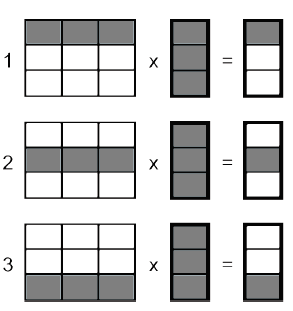
\includegraphics[width=0.5\textwidth]{pic}
\end{center}
Если число процессоров \textbf{p} меньше числа базовых подзадач \textbf{m},  базовые подзадачи могут быть укрупнены с тем, чтобы каждый процессор выполнял несколько операций умножения строк матрицы \textbf{А} и вектора \textbf{b}. В этом случае, по окончании вычислений каждая базовая подзадача будет содержать набор элементов результирующего вектора \textbf{с}.
\\\\
Распределение подзадач между процессорами вычислительной системы может быть выполнено с учетом возможности эффективного выполнения операции сбора данных.

\section{\LARGE Примеры решения}
Поясним выполнение метода сопряженных градиентов на примере решения системы линейных уравнений вида:
\begin{equation*}
	\begin{cases}
	3x_0 - x_1 = 3\\
	-x_0 + 3x_1 = 7\\
	\end{cases}
\end{equation*}
На первой итерации было получено значение градиента $g^1 = (-3, -7)$ , значение вектора направления $d^1 = (3, 7)$, значение величины смещения $s^1 = 0.439$.
\begin{itemize}
	\item [--] Соответственно, очередное приближение к точному решению системы $x^1=(1.318, 3.076)$.
\end{itemize}
На второй итерации было получено значение градиента $g^2=(-2.121, 0.909)$ ,значение вектора направления $d^2=(2.397, -0.266)$, а величина смещения $s^2=0.284$.
\begin{itemize}
	\item [--] Очередное приближение $x^2=(2, 3)$ совпадает с точным решением системы $x^*$.
\end{itemize}

Итерации метода сопряженных градиентов при решении системы второго порядка.
\begin{center}
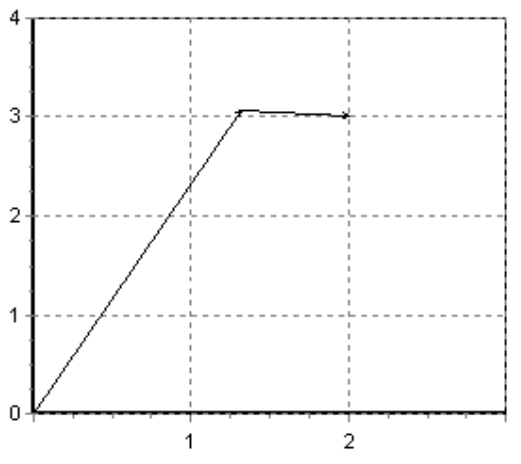
\includegraphics[width=0.5\textwidth]{g1}
\end{center}

\textbf{Пример №2 для СЛАУ 3-его порядка: }
\begin{equation*}
	\begin{cases}
	4x_0 -x_1 + 2x_2 = -1\\
	-x_0 + 6x_1 - 2x_2 = 9\\
	2x_0 - 2x_1 + 5x_2 = -10\\
	\end{cases}
\end{equation*}
Возьмем начальный вектор $x_0$ равным: 
\begin{center} 
	$x_0$ 
	= 
	$\begin{pmatrix}
  	1\\
  	0\\
  	0\\
  	\end{pmatrix}$
\end{center}
На первой итерации было получено значение градиента $g^1$ = (5,-10, 12) , значение вектора направления $d^1$ = (1.4086366 , -0.53557677, -1.37480788), значение величины смещения $s^1$ = 2.0245, очередное приближение к точному решению системы:
$x^1$ = (0.39955357  1.20089286 -1.44107143)\\ 
\\
На второй итерации было получено значение градиента $g^2$ = (-1.48482143, 0.68794643,  1.19196429) , значение вектора направления $d^2$ = (0.07722983, 0.0834236,  0.03615877), значение величины смещения $s^2$ = 0.1191, очередное приближение к точному решению системы:
$x^2$ = (0.98123643  0.97973161 -2.00878504)\\ 
\\
На третьей итерации было получено значение градиента $g^3$ = (1.48492330e-15, -2.42861287e-15,  2.37310172e-15) , значение вектора направления $d^3$ = (1.48492330e-15, -2.42861287e-15,  2.37310172e-15), значение величины смещения $s^3$ = 0.0000, очередное приближение к точному решению системы:
$x^3$ = (1.  1. -2)\\ 
\\
Получили корни, удовлетворяющие уравнениям системы.

\section{\LARGE Анализ эффективности}
\begin{itemize}
	\item [--]Вычислительная сложность параллельных операций умножения матрицы на вектор при использовании схемы ленточного горизонтального разделения матрицы составляет (здесь и далее $\mathbf{L}$ – количество итераций, выполняемых методом)
\begin{align*}
T^1_p(calc) &= L \cdot \frac{2n \cdot (2n - 1)}{p} \cdot \tau
\end{align*}
	\item [--]Все остальные операции над векторами (скалярное произведение, сложение, умножение на константу), также выполняются в многопоточном режиме. \\Следовательно, общая вычислительная сложность параллельного варианта метода сопряженных градиентов является равной:
\begin{align*}
T_p(calc) &= L \cdot \frac{4n^2 + 11n}{p} \cdot \tau 
\end{align*}
	\item [--]Общее время выполнения алгоритма в худшем случае составляет:
\begin{align*}
T_p &= L \cdot \frac{4n^2 + 11n}{p} \cdot \tau + L \cdot (2n^2 + 14n) \cdot (\alpha + \frac{64}{\beta})
\end{align*}
	\item [--]Для построения точной модели необходимо также учесть
коэффициент кэш промахов:
\begin{align*}
T_p &= L \cdot \frac{4n^2 + 11n}{p} \cdot \tau + \gamma \cdot L \cdot (2n^2 + 14n) \cdot (\alpha + \frac{64}{\beta})
\end{align*}
\end{itemize}
Общая оценка показателей ускорения и эффективности:
\begin{align*}
S_p &= \frac{2n^2 + 14n}{n(2[\frac{n}{p}] \cdot (2n-1) + 13n)},
E_p &= \frac{2n^2 + 14n}{p \cdot n(2[\frac{n}{p}] \cdot (2n-1) + 13n)}
\end{align*}

\section{\LARGE Результаты вычислительных экспериментов}
Параметры оборудования: Intel Core 2 Duo CPU E8500,  3.16 GHz, 2048MB RAM.\\\\
Длительность $\tau$ базовой скалярной операции - 0.0000000015 сек\\\\
Параметры передачи между процессами на одной машине: латентность $\alpha$ - 0.000024 сек, пропускная способность $\beta$ - 267506473 байт/сек
\begin{itemize}
	\item [--]График зависимости ускорения от количества исходных данных при выполнении параллельного метода сопряженных градиентов.
	\begin{center}
	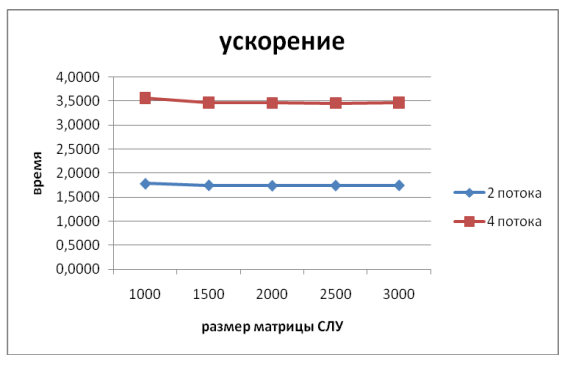
\includegraphics[width=\textwidth]{acc1}
	\end{center}
	\item [--]График зависимости экспериментального и теоретического времени выполнения параллельного алгоритма сопряженных градиентов от объема исходных данных при использовании \emph{двух потоков}: 
	\begin{center}
	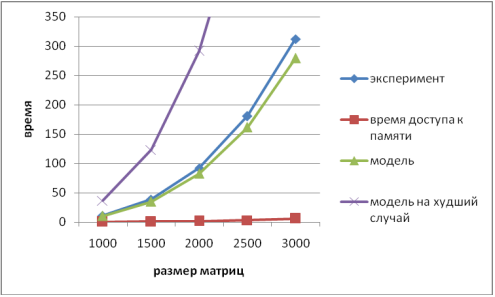
\includegraphics[width=\textwidth]{gra2}
	\end{center}
	\item [--]График зависимости экспериментального и теоретического времени выполнения параллельного алгоритма сопряженных градиентов от объема исходных данных при использовании \emph{четырех потоков}: 
	\begin{center}
	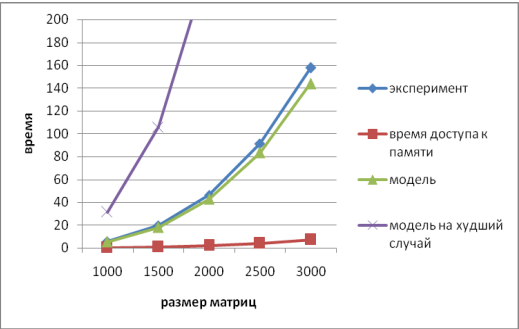
\includegraphics[width=\textwidth]{gra3}
	\end{center}
\end{itemize}

\textbf{Таблицы: }


\begin{center}
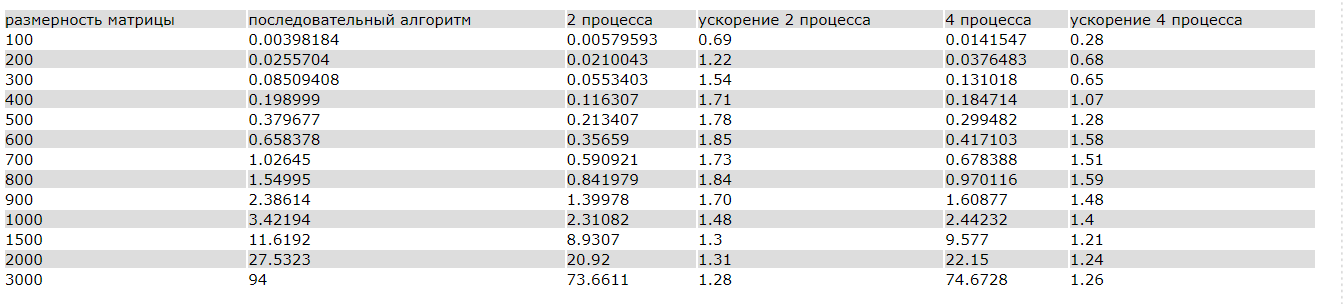
\includegraphics[width=1.2\textwidth]{table1}
\end{center}
Таблица сравнения времени экспериментов с модельным временем:
\begin{center}
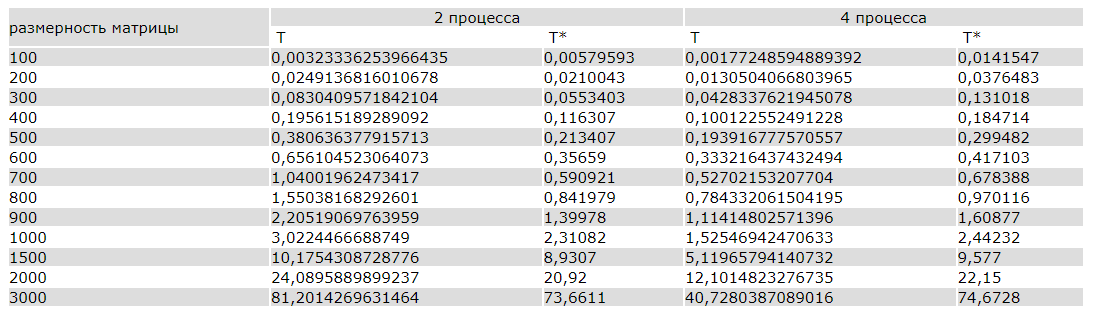
\includegraphics[width=1.2\textwidth]{table2}
\end{center}

\section{\ Вывод}
При рассмотрении параллельного варианта метода сопряженных градиентов, распараллеливание было произведено через параллельные алгоритмы выполняемых вычислительных действий – операций умножения матрицы на вектор, скалярного произведения векторов, сложения и вычитания векторов.
Такой подход позволил организовать параллельные вычисления с достаточно высокими показателями эффективности.
\end{document}
